\chapter{Axion--Like Particles search with ultracold neutrons}

\label{ch:axions}

\section{Motivation}


\section{Theoretical background}


\section{Time series construction}

\subsection{nEDM @ PSI data taking scheme}
The nEDM experiment at PSI probes the Ramsey resonance curve of ultra--cold neutrons (\emph{UCNs}). Its operation consists of subsequent \emph{cycles}, wherein an ensemble of polarised \emph{UCNs} undergoes a Ramsey cycle in a magnetic field. At the end the polarisation of the ensemble is measured. The measurement is performed in a controllable electric field, which takes up three values: parallel to the magnetic field, antiparallel to it and zero. The electric field configuration is altered every couple of tens of cycles.

The Ramsey resonance curve of the neutrons is probed only in four \emph{working points}, as shown in Fig.\,\ref{fig:axions_working_points}. The points lie on the curve's steep slope. Thereby the resonance position is determined more precisely then it would should the curve be probed homogeneously or close to the resonance.

\begin{figure}[bth]
  \myfloatalign
  \subfloat
  [The \emph{working points} method. The plot depicts the measured neutron polarisation in function of the $pi/2$ pulses frequency. The frequencies are normalised by appropriate gyromagnetic ratios.]
  {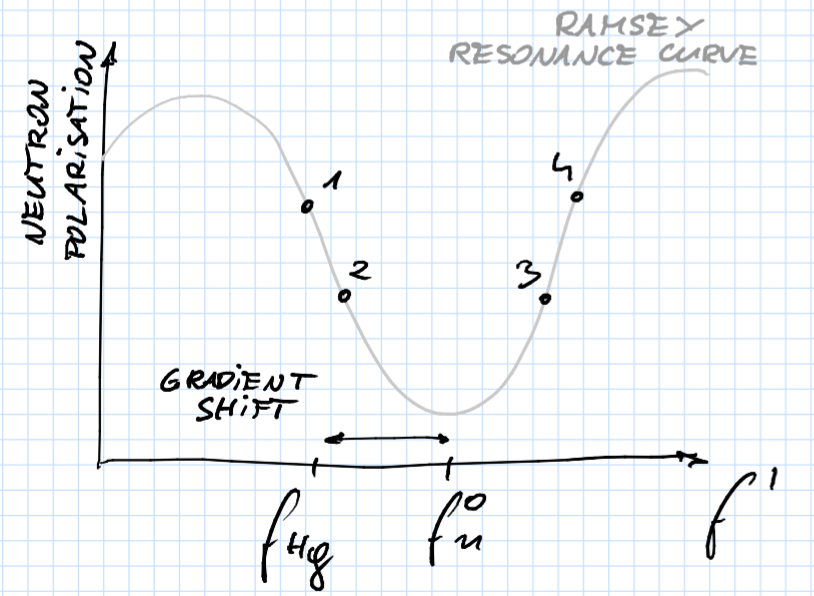
\includegraphics[width=.45\linewidth]{gfx/axions/data_taking_working_points}}
  \quad
  \subfloat
  [The \emph{working points} are probed subsequently.]
  {\label{fig:example-b}
  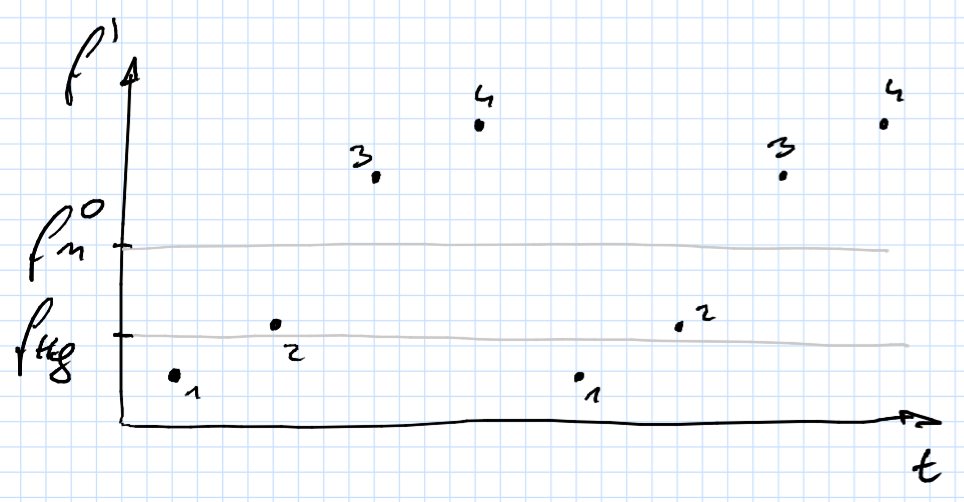
\includegraphics[width=.45\linewidth]{gfx/axions/data_taking_working_points_time}}
  \caption{The principle of working points}
  \label{fig:axions_working_points}
\end{figure}

The resonance frequency $f_n^{\,0}$ is determined with a fit of the resonance curve. Because the points are probed one after another, it is only possible after a set of data points, \emph{cycles}, have been measured. In order to extract the neutron precession frequency for each individual \emph{cycle}, one assumes that the only parameter of the resonance curve that varies on a cycle--to--cycle basis is the position of the resonance. With this assumption the shape of the curve, fitted to the whole set of \emph{cycles}, is used to calculate back the resonant frequency in each \emph{cycle} of the set.

Together with the UCNs there is a polarised $^{199}$Hg gas precessing. Its precession is monitored with light, allowing for direct determination of the $^{199}$Hg Larmor frequecy and thus the magnetic field strength. In order to cancel the first-order magnetic field changes one looks at the value:
\begin{equation}
  R := f_n / f_{Hg} \ .
\end{equation}
However, the UCNs are cold enough to have their centre of mass shifted downwards a few centimeters by the gravity. The $^{199}$Hg gas, being much hotter then the UCNs, fills the precession volume homogeneously. In a presence of a vertical magnetic field gradient this causes the two species to see different magnetic fields.

In the nEDM experiment at PSI data taking is divided into \emph{runs}. A single \emph{run} is carried out automatically with, in most cases, no human intervention. The machine cycles through the working points by itself. Also the charging of the electrodes creating the electric field is automatised. In between \emph{runs} manual interference happens, most importantly the magnetic field vertical gradient is altered.

In order to mitigate the bias due to the human factor, the nEDM experiment implements \emph{data blinding}. The data is artificially altered in a way that mimics a non--zero neutron electric dipole moment, big enough to be visible in the data. The exact value is secret and will be revealed only after the analysis is complete.


\subsection{An oscillating nEDM signal}
The main purpose of the experiment is to measure the constant neutron electric dipole moment. This would appear as a shift in $R$ dependent on the electric field. Zero electric field would cause no shift, while the parallel and anti--parallel configurations of the magnetic and electric fields would shift $R$ in opposite directions. Due to the \emph{data blinding} the shift is expected even in case of zero nEDM.

Should the neutron electric dipole moment oscillate, $R$ would oscillate as well. Even if the electric field is kept constant. A reversal of the electric field polarity would change phase of the oscillations by $\pi$. At zero electric field no oscillations would be visible. The effect is depicted in Fig.\,\ref{fig:axions_data_taking_one_run}.

\begin{figure}[bth]
  \myfloatalign
  \subfloat
  [An oscillating neutron electric dipole moment signal in the nEDM @ PSI apparatus. The colours indicate different electric field states: parallel to the magnetic field, antiparallel to it and zero]
  {\label{fig:axions_data_taking_one_run}
  % 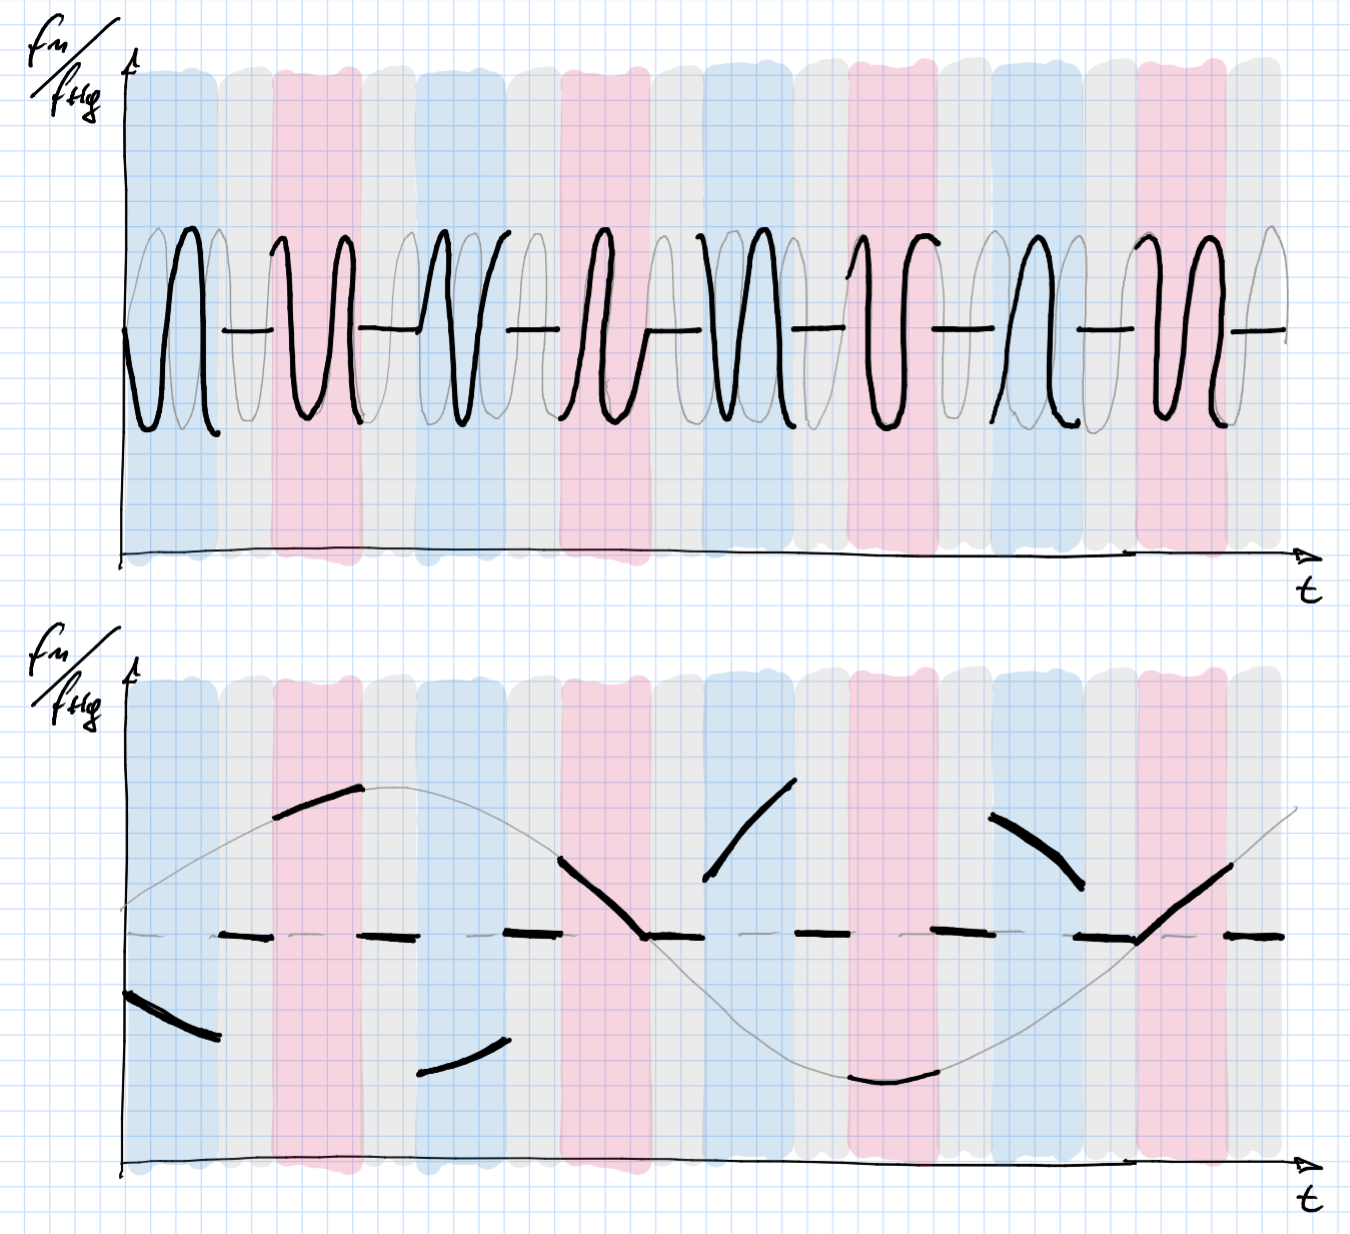
\includegraphics[width=.34\linewidth]{gfx/axions/data_taking_run}}
  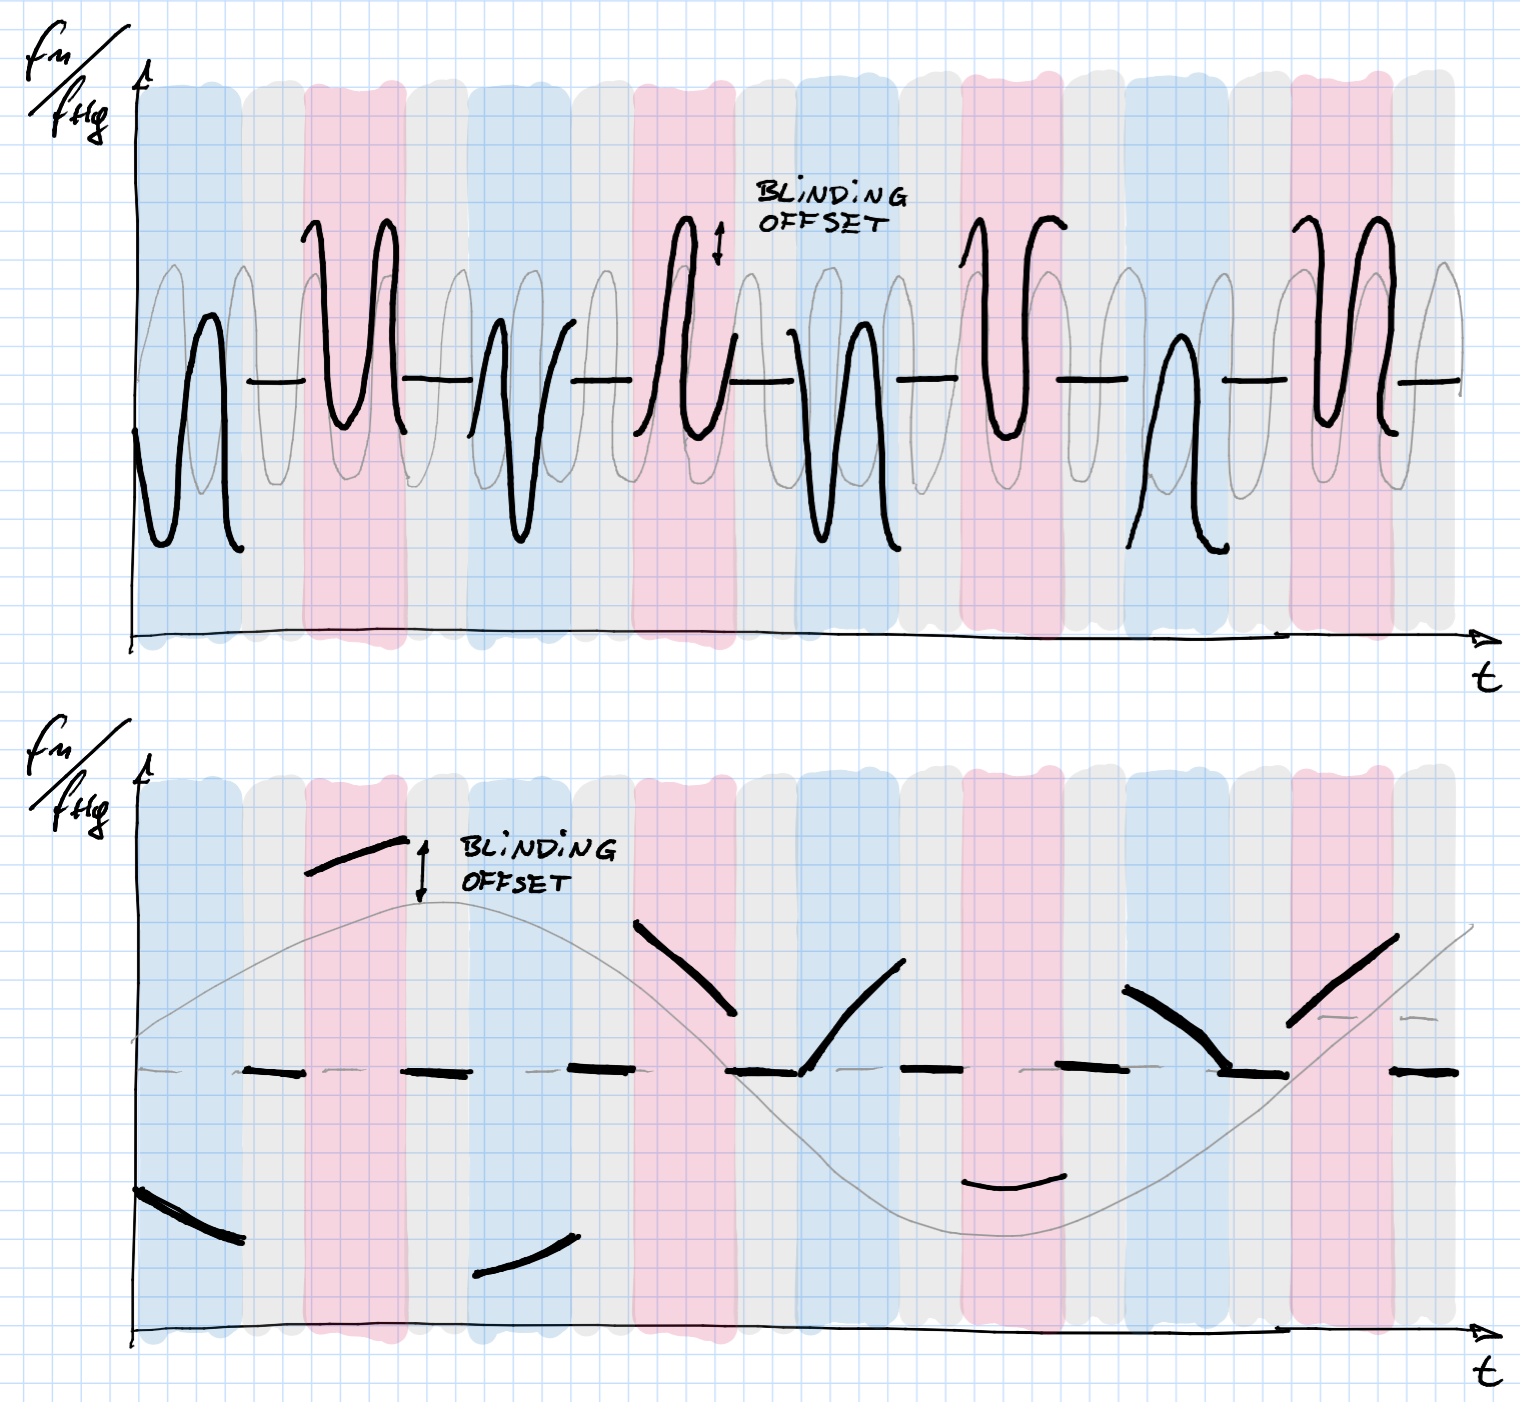
\includegraphics[width=.34\linewidth]{gfx/axions/data_taking_run_with_blinding}}
  \quad
  \subfloat
  [An oscillating neutron electric dipole moment signal in the nEDM @ PSI apparatus across many runs. The colours indicate different electric field states: parallel to the magnetic field, antiparallel to it and zero. Different runs have different magnetic field gradients, which causes each run to have a different shift in $R = f_n / f_{Hg}$.]
  {\label{fig:axions_data_taking_runs}
  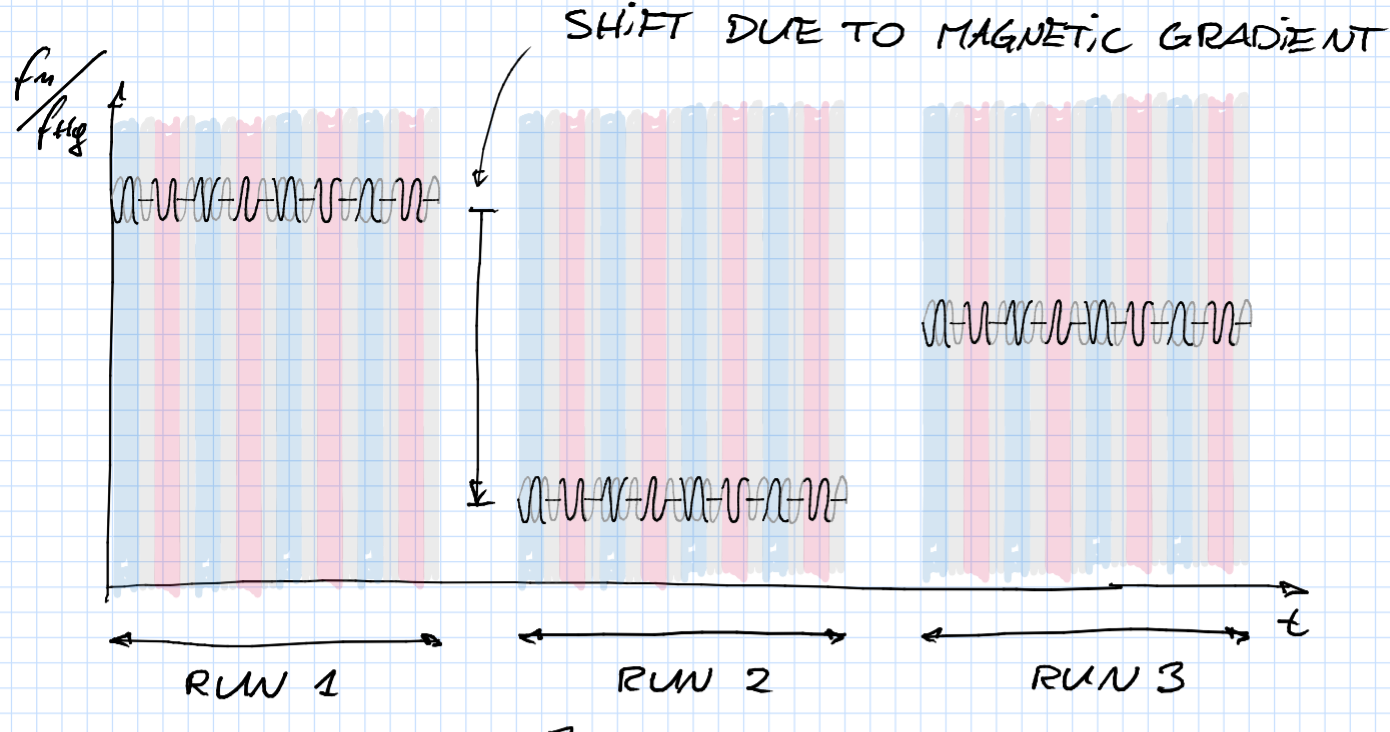
\includegraphics[width=.56\linewidth]{gfx/axions/data_taking_runs}}
  \caption{The data taking scheme in the nEDM experiment at PSI.}
\end{figure}

The vertical magnetic filed vertical gradient changes when a new \emph{run} is started. Thereby $R$ is shifted by a big value, changing the DC level of the oscillating nEDM signal, which is illustrated in Fig.\,\ref{fig:axions_data_taking_runs}. Moreover, even during a single \emph{run} the gradient drifts, as clearly visible in Fig.\,\ref{fig:axions_gradient_drift}.

The nEDM team spares no effort to measure the gradient. Nevertheless, the achieved precision ($\approx \unit[1]{pT/cm}$ is only comparable to the one of $f_n$ (in the order of \unit[1]{pT}). The exact way how the gradient should determined is highly non--trivial and there is ongoing research in this respect. Actually, even the height difference between the neturons and $^{199}$Hg centres of mass (a few milimeters) is still discussed. % Assuming a constant gradient during a \emph{run} one can determine it much more precise. This assumption, however, is known not to be exactly true.

\begin{figure}[bth]
  \myfloatalign
  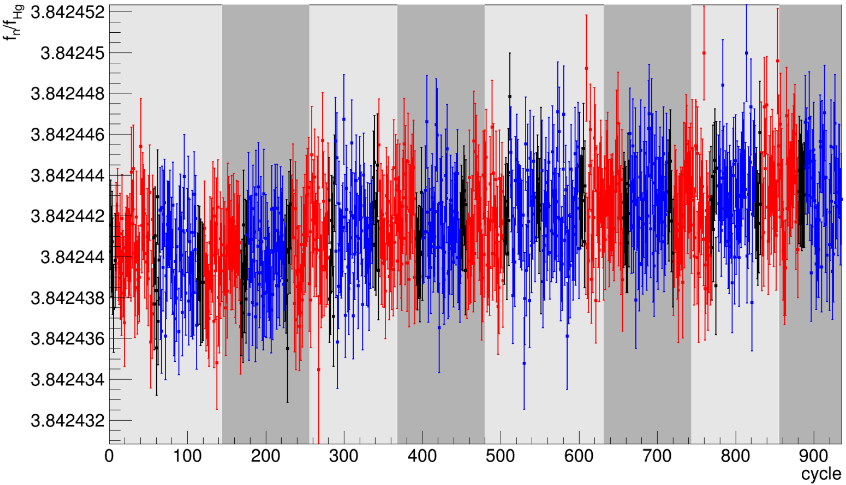
\includegraphics[width=.8\linewidth]{gfx/axions/gradient_drift_yoann}
  \caption
  [Drift of $R$]
  {%FIXME directly copied from Yoann's presentation on the 2015 PSI collaboration meeting
A typical time series of $R$ in the nEDM experiment. The colours depict electric field states, black being no electric field. A drift is clearly visible.}
  \label{fig:axions_gradient_drift}
\end{figure}

One should note, that any, including an oscillating one, nEDM effect affects only the position of the neutrons' resonance. The shape of the resonance curve is unaffected. Therefore, the method to extract neutron Larmor frequency $f_n$, and thereby $R$, for each \emph{cycle} is valid also in case of an oscillating nEDM.


\subsection{$R$ time series demodulation}
The time series of $R$ is not eligible for a Fourier--type analysis. The series has to be first demodulated into a coherent signal. To accound for the electric field changes, data taken at one configuration need to be \emph{flipped} around the DC level. Unfortunately, determining the DC level is not trivial.

Taking a look at Fig.\,\ref{fig:axions_gradient_drift} it becomes clear, that the $R$ value drifts. The main reason is a drift of the vertical gradient of the magnetic field. This effect could corrected for using the gradient measurement, as shown in Fig.\,\ref{fig:axions_gradient_drift_correction}. It is not straightforward, though, as there is not yet an established method to determine the gradient. The points taken at zero electric field provide additional information about the DC level. This, however, would have to be interpolated. The gradient drift correction is likely to turn out to be the most delicate part of the analysis.

\begin{figure}[bth]
  %FIXME directly copied from Elise's presentation on the 2015 PSI collaboration meeting
  \myfloatalign
  \subfloat
  [Another time series of $R$ in the nEDM experiment. The colours depict electric field states, black being no electric field. A drift is clearly visible.]
  {\label{fig:axions_gradient_drift_not_corrected}
  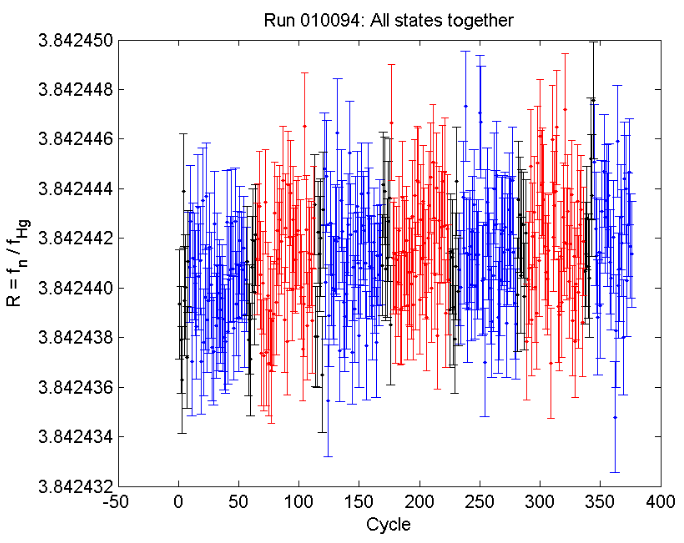
\includegraphics[width=.45\linewidth]{gfx/axions/gradient_drift_elise}}
  \quad
  \subfloat
  [The data as on Fig.\,\ref{fig:axions_gradient_drift_not_corrected} corrected for gradient fluctuations.]
  {\label{fig:axions_gradient_drift_corrected}
  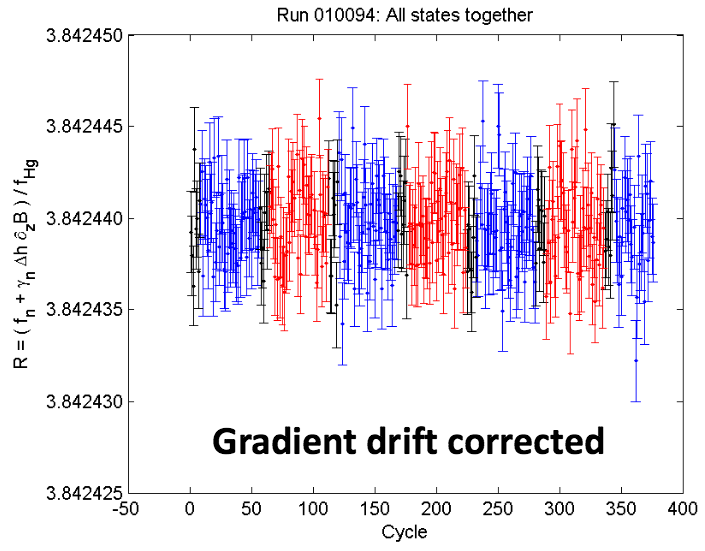
\includegraphics[width=.45\linewidth]{gfx/axions/gradient_drift_elise_corrected}}
  \caption{Correcting the $R$ time series for fluctuations of the vertical magnetic field gradient.}
  \label{fig:axions_gradient_drift_correction}
\end{figure}

% The gradient drift correction is likely to turn out to be the most delicate part of the analysis. One could consider two methods of tackling the problem. Firstly, the electric field configurations could be separated and analysed separately. In this case no correction for the gradient drift is necessary, although it
%
% Because of drift - not trivial to correct.
% Two analyses:
% 1. + and - HV separately -- the highest freqency is twice slower, but no correction necessary, but still possible. Gradient drift mimics a signal though.
% 2. try to correct for gradient and combine the data into one array


\section{Time series analysis}
\subsection{Definition of the periodogram}
The analysis starts with calculating \emph{the periodogram}, an estimator of the power spectral density, of the demodulated $R$ time series. Therefor an array of $N$ frequencies $\omega_i$ is chosen. For each a linear least--squares fit is performed with a model:
\begin{equation}
  R(t) = A\ \mathrm{sin}\,\omega t + B\ \mathrm{cos}\,\omega t \ .
\end{equation}
Then the power at the frequency $\omega$ is defined:
\begin{equation}
  P(\omega) = \frac{N}{4} \, (A^2 + B^2)\ .
\end{equation}
The definition is similar to the one used by \citeauthor{VanTilburg2015}~\citep{VanTilburg2015}, but uses normalisation as defined by \citeauthor{Scargle1982}~\citep{Scargle1982}. One should remember, that the periodogram is an estimator. Its statistical properties are thoroughly described by \citeauthor{Scargle1982}~\citep{Scargle1982}.


\subsection{Null hypothesis test}
Once the periodogram of the real data, demodulated $R$ time series, is calculated we look for a signal. A signature of a periodic signal is a peak in the periodogram. The really interesting statement is the answer to the question:

\begin{center}
  \emph{How likely it is, that the highest peak in the periodogram cannot be only a random fluctuation?}
\end{center}

To describe the question mathematically, let us denote the time series from the real data by $D$. The peridogoram is then a set of $P^D(\omega_i)$. We are interested in \emph{the maximum of the periodogram}:
\begin{align}
  P_{max}^D &:= \mathrm{max}_i\,P^D(\omega_i) \\
  \omega_{max}^D &:= \mathrm{arg\,max}_i\,P^D(\omega_i)
\end{align}
The height of the maximum, $P_{max}^D$, is a random variable. We consider the distribution of $P_{max}$ given the null hypothesis, $H_0$, where an array of normally distributed random variables is taken. The probability that a peak at least as high as the one observed arises as a random fluctuation is:
\begin{equation}
  \mathrm{Pr}\left( P_{max} > P_{max}^D\ |\, H_0 \right) \ .
\end{equation}
This value is called the \emph{false alarm probability} (see eg. \citeauthor{Pandola2004}~\citep{Pandola2004}). It can be numerically calculated with a Monte--Carlo method by generating random data according to the null hypothesis and counting the relative number of cases when $P_{max} > P_{max}^D$. To claim a discovery the \emph{false alarm probability} has to be at most in the range of $10^{-7}$ (so--called 5--sigma).

It should be stressed that the distribution of $P_{max}$ is very different from the distribution of $P(\omega_{max})$. The highest peak will always occur in a far tail of the $P(\omega_{max})$ distribution, which is natural. By looking for the highest peak we check a big number of random variables $P(\omega_i)$ and pick the one that does lie the furthest in the tail of the distribution. The distribution of $P_{max}$ is centered around much higher values, as the highest peak is bound to occur \emph{somewhere}. It is explained in Fig.\,\ref{fig:axions_null_rejection}.

\begin{figure}[bth]
  \myfloatalign
  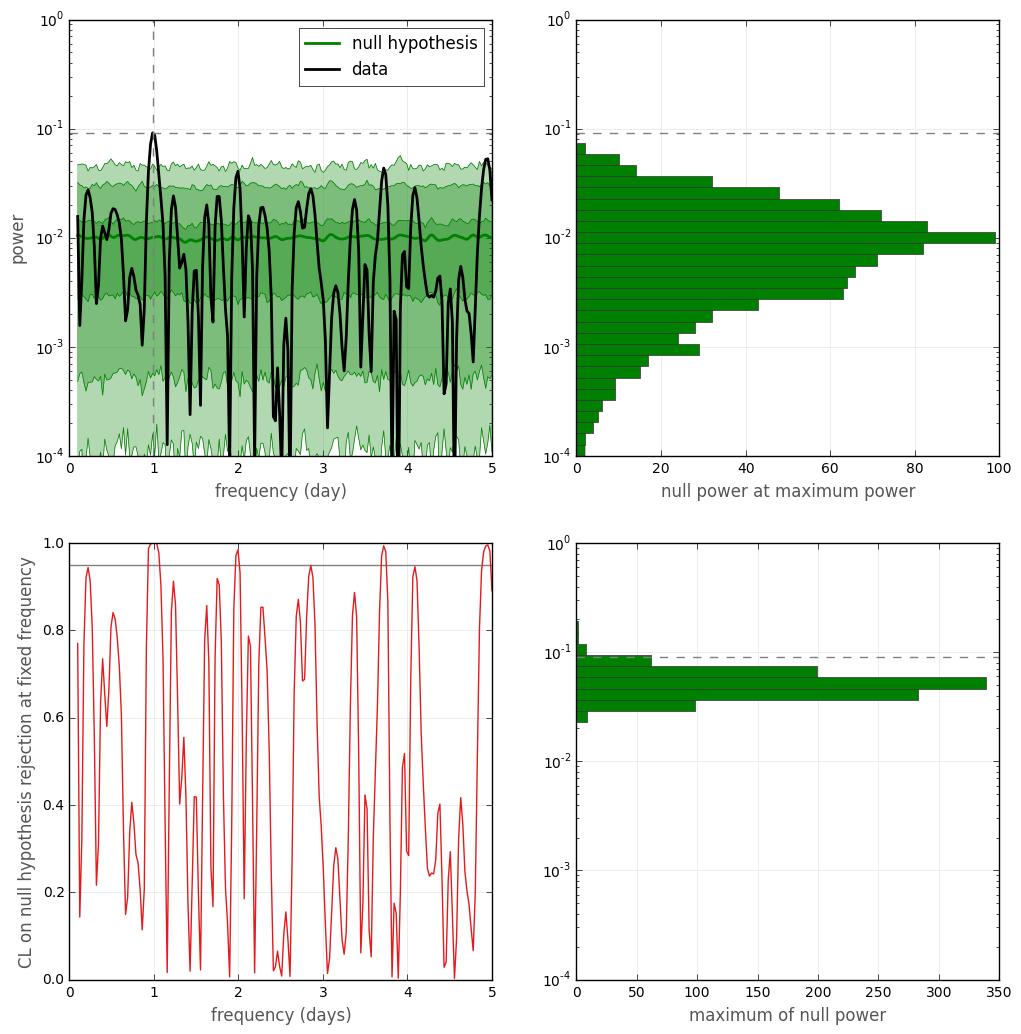
\includegraphics[width=.8\linewidth]{gfx/axions/axionMC_null_rejection}
  \caption
  [...]
  {
Testing not--yet--real data against the null hypothesis. \textsc{Upper--left:} The periodogram of the data (black line) on top of the periodogram of the null hypothesis (green line with Monte--Carlo generated distribution bands). \textsc{Upper--right:} The distribution of $P(\omega_{max})$, given the null hypothesis (vertical slice through the green part of the plot in the upper--left corner). \textsc{Lower--left:} CDF of $P(\omega)$ evaluated at $P^D(\omega)$ in function of $\omega$. \textsc{Lower--right:} The distribution of $P_{max}$. }
  \label{fig:axions_null_rejection}
\end{figure}


\subsection{Signal hypotheses tests}
Should no claim for a discovery be possible, the next question to ask is:
\begin{center}
  \emph{Which oscillations would produce a visible peak, but did not, and can be thus excluded?}
\end{center}
In order to answer this question, the data need to be tested against being compatible with a number of model signal hypotheses. As an oscillation is characterised by its amplitude and frequency, the space of the hypotheses to test is two--dimensional.

The probability that a hypothetical oscillation of amplitude $A$ and frequency $\omega$ would produce more power at $\omega$ then observed is:
\begin{equation}
  \mathrm{Pr}\left( P(\omega) > P^D(\omega)\ |\, H(\omega, A) \right) \ .
\end{equation}
This probability is the \emph{confidence level} (C.L.) at which the hypothesis $H(\omega, A)$ can be rejected. Figure\,\ref{fig:axions_signal_rejection} presents comparing a not--yet--real data power spectrum with a hypothetical signal. This test may be performed many times, each covering a \emph{pixel} of the space of possible hypotheses, forming an image as in Fig.\,\ref{fig:axions_exclusion}. The set of hypotheses excluded at a certain C.L. (often 95\%) forms an \emph{exclusion region}.

\begin{figure}[bth]
  \myfloatalign
  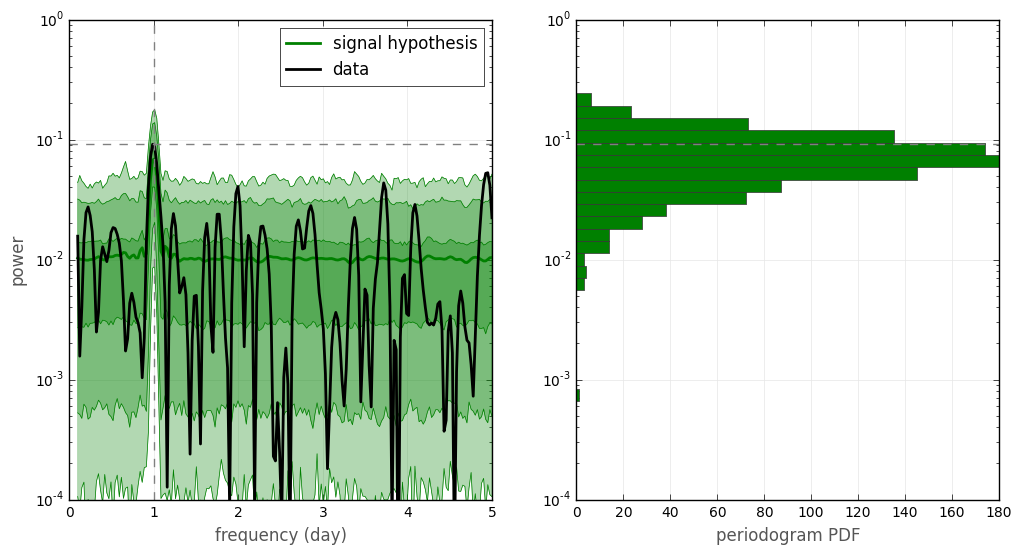
\includegraphics[width=.8\linewidth]{gfx/axions/axionMC_signal_hypothesis_rejection}
  \caption
  [...]
  {
\textsc{Left:} A periodogram of not--yet--real data on top of distribution of a periodogram of a hypothetical signal (green). \textsc{Right:} The distribution of power of the hypothetical signal at its model frequency.}
  \label{fig:axions_signal_rejection}
\end{figure}

\begin{figure}[bth]
  %FIXME directly copied from Elise's presentation on the 2015 PSI collaboration meeting
  \myfloatalign
  \subfloat
  [The not--yet--real data tested against hypothetical signals. Each pixel is one signal hypothesis. The white line connects points of 95\% C.L., surrounding an exclusion region. Note how deep into low amplitudes the line goes for couple of frequencies. See the text for the explanation.]
  {\label{fig:axions_exclusion}
  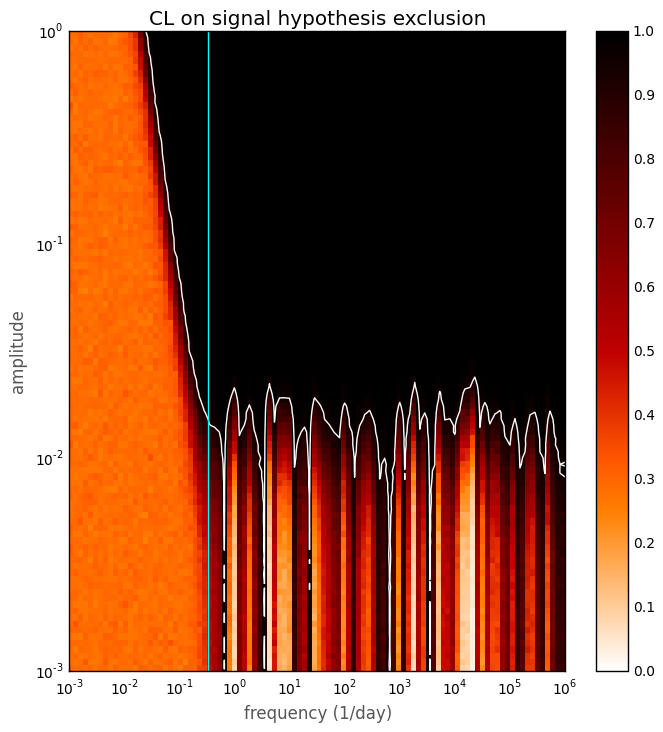
\includegraphics[width=.45\linewidth]{gfx/axions/axionMC_exclusion}}
  \quad
  \subfloat
  [The not--yet--real data tested against hypothetical signals using the \emph{CLs method}, in which hypotheses to which the experiment is not sensitive to get a statistical penalty. ]
  {\label{fig:axions_exclusion_CLs}
  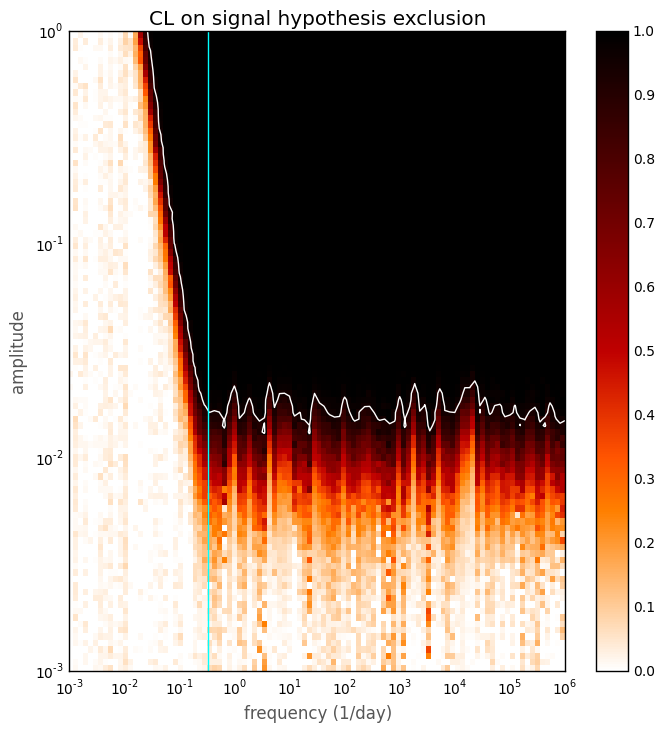
\includegraphics[width=.45\linewidth]{gfx/axions/axionMC_exclusion_CLs}}
  \caption{Exclusion region --- signals that can be excluded at 95\% confidence level.}
  \label{fig:axions_exclusions}
\end{figure}

The exclusion region, depicted by a white line in Fig.\,\ref{fig:axions_exclusion}, is exhibits a number of thin peaks going down in very low amplitudes. Seemingly for some frequencies signals with amplitude far below the sensitivity of the experiment are excluded. This is disturbing. Consider, however, that as the power was evaluated for many frequencies, inevitably at some of them, roughly 5\%, the power is low enough to be rejected at 95\%~C.L. even when tested against a white noise. However completely fine from the statistical point of view, physicists do not accept a situation, where a hypothesis is rejected based on an experiment which was not sensitive to it. One possible solution is called the \emph{CLs method}. The method is defined, as well the problem itself discussed, in the booklet of Particle Data Group~\citep{Group2014}. With use of the \emph{CLs method} the exclusion final region is obtained, as shown in Fig.\,\ref{fig:axions_exclusion_CLs}.


\section{Dedicated measurement}
One could consider performing a dedicated measurement for the ALP search. With a short, more densely sampled measurement one could explore the high mass (thus high frequency) region of possible axions, as was done eg. by \citeauthor{VanTilburg2015}~\citep{VanTilburg2015}.

The measurement would not need to last longer then a day. More dense sampling is possible by shortening the length of a \emph{cycle}. One should note that this worsens at the same time the sensitivity of the measurement. The lowest possible period of measurement in the nEDM apparatus is around \unit[100]{s}.

\section{Results}
